% !TEX program = pdflatex
% PRL-format theory draft. Numerical details and audit tables are in suppl.tex.
\documentclass[aps,prl,reprint,superscriptaddress,nofootinbib]{revtex4-2}

\usepackage[T1]{fontenc}
\usepackage{lmodern}
\usepackage{microtype}
\usepackage{amsmath,amssymb,bm}
\usepackage{graphicx}
\usepackage[hidelinks]{hyperref}

\hypersetup{
  pdftitle={A strict Rayleigh bound state in the continuum in a two-groove underwater acoustic metagrating},
  pdfauthor={Author names to be inserted},
  pdfsubject={Theory of acoustic Rayleigh-threshold bound states in the continuum}
}

\newcommand{\ii}{\mathrm{i}}
\newcommand{\e}{\mathrm{e}}
\newcommand{\BIC}{\mathrm{BIC}}
\newcommand{\RA}{\mathrm{RA}}
\providecommand{\hom}{\mathrm{hom}}
\providecommand{\dr}{\mathrm{dr}}

\begin{document}

\title{A strict Rayleigh bound state in the continuum in a two-groove underwater acoustic metagrating}
\author{Author Name}
\affiliation{Affiliation to be inserted}
\author{Coauthor Name}
\affiliation{Affiliation to be inserted}
\date{\today}

\begin{abstract}
At a Rayleigh threshold, zero normal flux does not by itself imply a bound
state: a finite grazing pressure remains non-square-integrable.  We construct
a strict Rayleigh-threshold bound state in the continuum in a rigid,
two-groove underwater acoustic metagrating, with both groove widths exceeding
$1$~mm.  At $200$~kHz in water, the state occurs at
$(\kappa,\Omega)=(0.083848696553,0.916151303447)$, or
$\theta=\pm5.251216^{\circ}$.  For positive angle the finite-flux $n=0$
amplitude and the grazing $n=-1$ amplitude both vanish.  The reduced
homogeneous operator has singular-value ratio $1.26\times10^{-15}$, while an
unconstrained full-operator calculation at the same endpoint gives
$7.72\times10^{-16}$.  A same-geometry complex-pole continuation reaches the
endpoint with a local finite-model $Q\sim|\Delta\kappa|^{-1.996}$ trend.
Homogeneous fields verify exterior localization, and two independent aperture
phasors cancel the two radiation constraints.  A single large rectangular
cavity remains at residual $0.125$ within the searched family.  Random
dimensional perturbations show that the strict cancellation is fabrication
sensitive.  All results refer to an infinite, rigid, lossless modal model.
\end{abstract}

\maketitle

A bound state in the continuum (BIC) is a localized eigenstate at a real
frequency embedded in propagating radiation channels.  It is defined by the
vanishing coupling of a \emph{homogeneous} mode to every radiative channel,
not by a dip in a driven reflectance spectrum
\cite{Hsu2016BIC,Koshelev2023Review,Azzam2021Review}.  Symmetry, destructive
interference, and topological charge provide established routes to photonic
BICs \cite{Yang2014Analytical,Zhen2014Topological}; trapped-light observations
and perturbative pole analyses show how leaky resonances approach such states
\cite{Hsu2013Observation,Sadrieva2017LeakyResonances,Abdrabou2022FrequencyPerturbation}.

A diffraction threshold requires stricter bookkeeping.  When a Floquet order
opens, its normal wavenumber and normal power flux vanish, but a nonzero
pressure amplitude is independent of the surface-normal coordinate and is
therefore not square-integrable.  The singular structure of scattering
matrices at channel openings is well known
\cite{Rayleigh1907,Wojcik2021ThresholdScattering}; at such a point, a strict
BIC must cancel the threshold \emph{amplitude} as well as every finite-flux
open amplitude.  The recent electromagnetic Rayleigh-BIC construction frames
this event as a resonant pole reaching a Rayleigh branch point
\cite{Karavaev2026Rayleigh}.

Acoustic metagratings offer compact, independently tunable cavity modes
\cite{Assouar2018AcousticMetasurfaces,Ni2019Splitter,Torrent2018Anomalous,Jin2019Grating}.
Waterborne implementations have demonstrated anomalous and negative-order
reflection \cite{Bernard2022NegativeReflection,Fan2021Multifunctional,Cao2024UnderwaterAbnormal},
and underwater resonant systems have exhibited high-$Q$ and merged-BIC
behavior \cite{Farhat2024UltrahighQ,Yang2024MergedFP}.  Here we ask a narrower
question: can an acoustic grating at a single Rayleigh opening support a
square-integrable homogeneous null when one additional diffraction order is
already propagating?  We answer this question constructively and test the
threshold coefficient directly.

Consider a sound-hard surface of period $a$ occupying $y\leq0$, with water in
$y>0$ and time dependence $\e^{+\ii\omega t}$.  For incidence toward the
surface and outgoing reflection,
\begin{align}
 p_{\mathrm{inc}}&=\e^{-\ii k_{x,0}x+\ii k_{y,0}y},
 &p_{\mathrm{sc}}&=\sum_{n\in\mathbb Z}A_n^{\dr}
 \e^{-\ii k_{x,n}x-\ii k_{y,n}y},                                      \label{eq:fields}\\
 k_{x,n}&=k_0\sin\theta+\frac{2\pi n}{a},
 &k_{y,n}&=\sqrt{k_0^2-k_{x,n}^2}.                                      \label{eq:wavenumbers}
\end{align}
The outgoing branch has $\Re k_{y,n}\geq0$ and $\Im k_{y,n}\leq0$.  We use
\begin{equation}
 \Omega=\frac{af}{c},\qquad
 \kappa=\frac{ak_0\sin\theta}{2\pi}=\Omega\sin\theta,\qquad
 |\kappa+n|=\Omega                                                       \label{eq:rayleigh}
\end{equation}
for a Rayleigh threshold of order $n$.

The optimized cell in Fig.~\ref{fig:structure} has
\begin{align}
 a&=6.871134776~\mathrm{mm},\qquad
 g=0.926658264~\mathrm{mm},\nonumber\\
 (d_1,d_2)&=(4.541418182,1.080580298)~\mathrm{mm},\nonumber\\
 (w_1,w_2)&=(3.964770159,1.053048089)~\mathrm{mm}.                       \label{eq:geometry}
\end{align}
At $f=200$~kHz and $c=1500$~m/s,
\begin{align}
 \kappa_{\BIC}&=0.083848696553,\qquad
 \Omega_{\BIC}=0.916151303447,\nonumber\\
 \theta_{\BIC}&=\pm5.251216^{\circ}.                              \label{eq:point}
\end{align}
For $+\theta$, $n=0$ is propagating, $n=-1$ is at threshold because
$\kappa+\Omega=1$, and $n=+1$ is evanescent.  Reversing the Bloch number
exchanges $n=-1$ and $n=+1$.

\begin{figure*}[t]
  \centering
  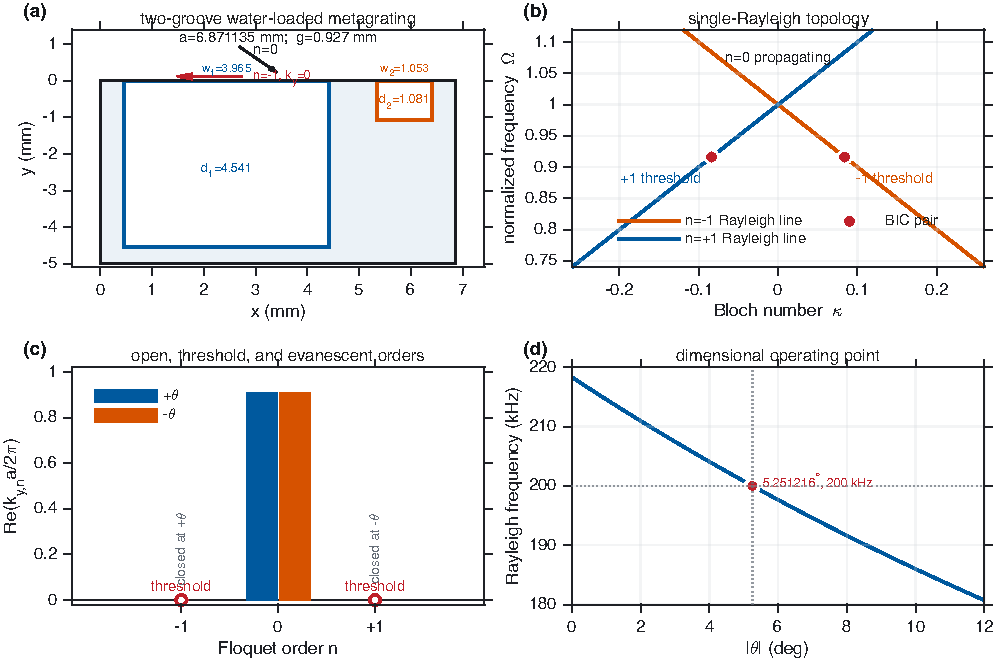
\includegraphics[width=\linewidth]{figures/fig1_structure_topology.pdf}
  \caption{\label{fig:structure}
  Geometry and channel topology.  (a) Final two-groove cell; dimensions are
  in millimeters.  (b) The two first-order Rayleigh lines and the reciprocal
  BIC pair.  The zeroth order is propagating at both points.  (c) Normal
  wavenumbers for the three displayed orders: for $+\theta$ ($-\theta$),
  $n=-1$ ($n=+1$) is grazing and the opposite first order is evanescent.
  (d) The positive-angle point on the dimensional $n=-1$ Rayleigh curve.}
\end{figure*}

\begin{figure*}[t]
  \centering
  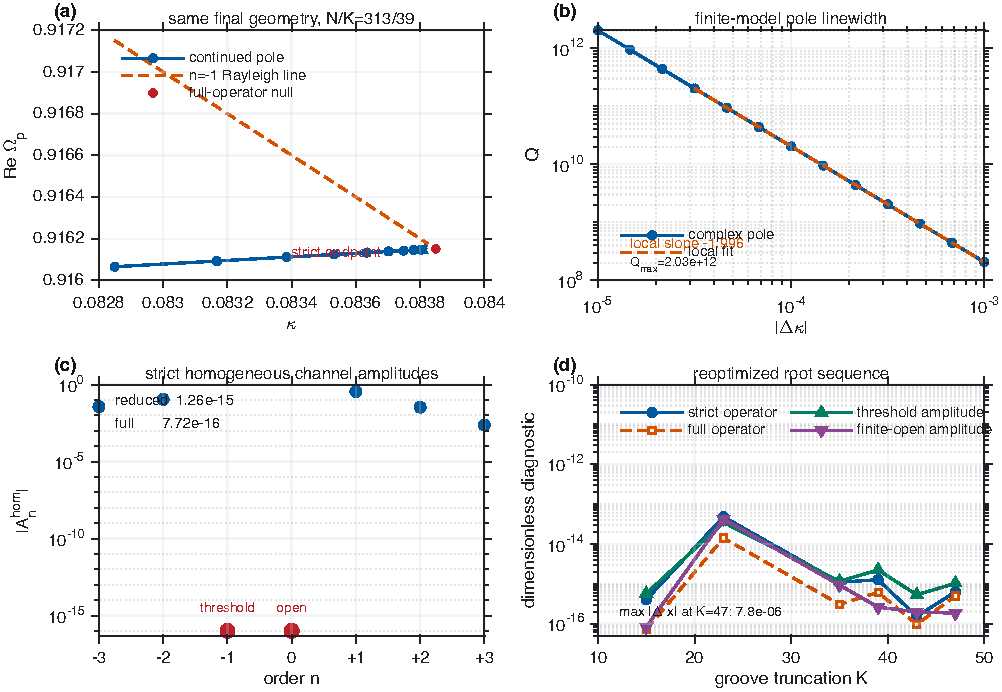
\includegraphics[width=\linewidth]{figures/fig2_strict_bic_evidence.pdf}
  \caption{\label{fig:evidence}
  Strict-null evidence.  (a) Final-geometry pole trajectory and the
  $n=-1$ Rayleigh line.  The red endpoint is also a null of the full
  $(313,39)$ operator.  (b) Pole quality factor and local fit; the exponent
  is a resolved finite-model trend.  (c) Final homogeneous Floquet
  amplitudes.  The finite-flux $n=0$ and threshold $n=-1$ coefficients
  vanish, while the displayed remaining orders are evanescent.
  (d) Reoptimized root sequence: reduced and full singular-value ratios and
  the independently extracted threshold/open amplitudes remain at machine
  precision through $(377,47)$.}
\end{figure*}

\begin{figure*}[t]
  \centering
  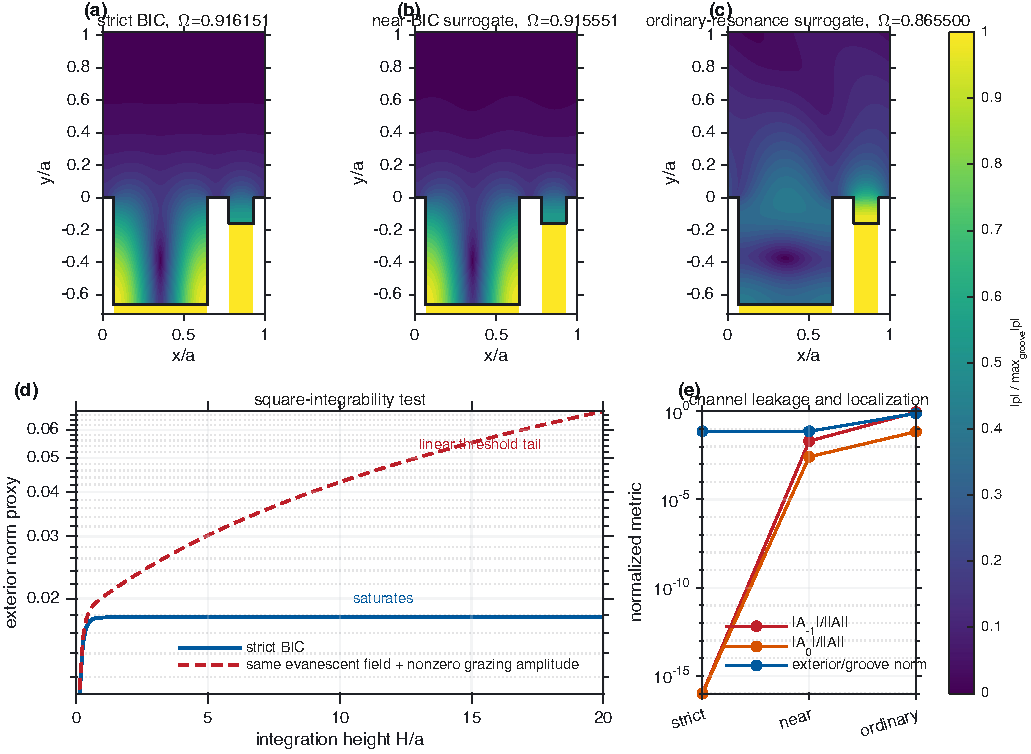
\includegraphics[width=\linewidth]{figures/fig3_homogeneous_fields.pdf}
  \caption{\label{fig:fields}
  Homogeneous pressure fields and localization.  (a) Strict BIC.
  (b) Near-BIC real-axis surrogate at $\Omega=0.9155513$.
  (c) Ordinary-resonance real-axis surrogate at $\Omega=0.8655$.
  All maps show $|p|/\max_{\mathrm{groove}}|p|$ on the same scale; white
  regions are rigid material.  (d) Exterior norm versus integration height
  for the strict mode and for the same evanescent field with a nonzero
  grazing component added.  (e) Threshold amplitude, finite-open amplitude,
  and exterior-to-groove norm proxies.  Panels (b,c) are diagnostic
  surrogates, not exact quasinormal-mode fields.}
\end{figure*}

\begin{figure*}[t]
  \centering
  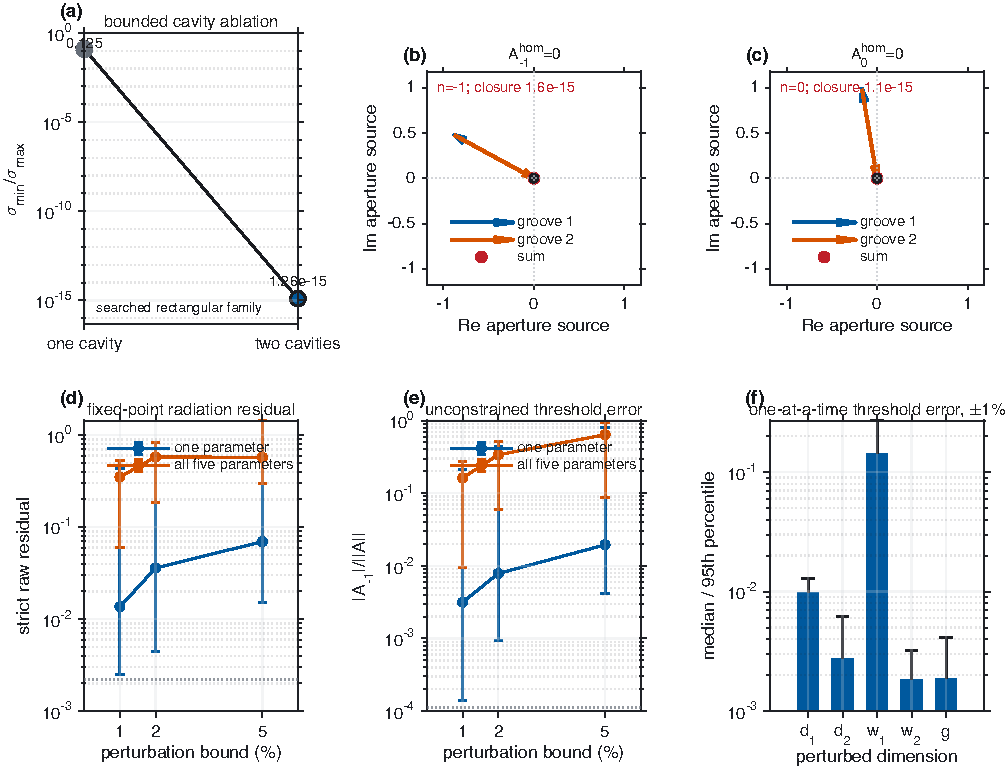
\includegraphics[width=\linewidth]{figures/fig4_dof_tolerance.pdf}
  \caption{\label{fig:mechanism}
  Cavity degrees of freedom and fixed-point sensitivity.
  (a) Best single-large-cavity result in the searched rectangular family
  versus the two-groove root.  (b,c) Separate aperture-source phasor closures
  for the grazing $n=-1$ and propagating $n=0$ constraints.
  (d,e) Medians and 5--95\% intervals of the strict raw residual and the
  unconstrained threshold-amplitude error for one-parameter and joint
  perturbations.  The dotted line is the unperturbed $(185,23)$ numerical
  floor.  (f) One-at-a-time $\pm1\%$ sensitivity; bars are medians and
  whiskers are 95th percentiles.}
\end{figure*}

Inside groove $\ell$, a bottom-rigid cosine expansion is retained.  Projecting
pressure and normal-velocity continuity without eliminating the groove
coefficients gives the pole-free homogeneous system
\begin{equation}
 \mathsf F(\omega,\kappa;\bm g)
 \begin{bmatrix}\bm A^{\hom}\\ \bm C\end{bmatrix}=0,
 \qquad \bm g=(d_1,d_2,w_1,w_2,g).                                      \label{eq:operator}
\end{equation}
The full block matrix, scaling, and driven reduction are given in the
Supplemental Material.  This separation is essential: $A_n^{\dr}$ contains
the forced background response, whereas $A_n^{\hom}$ belongs to an outgoing
eigenmode.

For a single homogeneous exterior order, define the height-integrated
pressure norm $\mathcal N_n(H)$ by
\begin{equation}
 \mathcal N_n(H)=\int_0^H |p_n^{\hom}|^2\,\mathrm{d}y.
 \label{eq:norm-definition}
\end{equation}
It evaluates to
\begin{equation}
 \mathcal N_n(H)=
 \begin{cases}
 H|A_n^{\hom}|^2,&k_{y,n}=0,\\[2pt]
 \dfrac{|A_n^{\hom}|^2}{2\alpha_n}
 (1-\e^{-2\alpha_nH}),&k_{y,n}=-\ii\alpha_n.
 \end{cases}                                                            \label{eq:norm}
\end{equation}
Thus the positive-angle state is strict only if
\begin{equation}
 A_{-1}^{\hom}=0,\qquad A_0^{\hom}=0.                                   \label{eq:strict}
\end{equation}
We first impose Eq.~\eqref{eq:strict} by removing those two amplitude columns
from the unknown vector, row- and column-scale the remaining operator, and
reconstruct its smallest right singular vector.  At $(N,K)=(313,39)$,
where $N$ is the number of exterior orders and $K$ is the cosine-mode count
per groove,
\begin{align}
 \sigma_{\min}/\sigma_{\max}&=1.2603643\times10^{-15},\nonumber\\
 r_{\mathrm{raw}}&=1.3765668\times10^{-13}.                         \label{eq:residual}
\end{align}
This constrained null is not the sole evidence.  Evaluating the complete
complex-frequency operator at the same final geometry, with the selected
$k_{y,-1}$ set exactly to zero, gives
$\sigma_{\min}/\sigma_{\max}=7.7151\times10^{-16}$ and an unconstrained null
whose open and threshold amplitudes vanish at machine precision.

The solution persists as a reoptimized sequence through
$(N,K)=(377,47)$; all strict and full-operator residuals remain at numerical
precision and the maximum normalized parameter step falls to
$7.77\times10^{-6}$.  This is evidence for a converging modal sequence, not a
formal continuum theorem.  A complex-pole continuation performed at the
\emph{same} final $(313,39)$ geometry stays on one branch with minimum
successive mode overlap $0.9999995$ and reaches
$Q=2.026\times10^{12}$ at $|\Delta\kappa|=10^{-5}$.  The resolved local fit is
$Q\propto|\Delta\kappa|^{-1.9959}$ [Fig.~\ref{fig:evidence}(b)]; we do not
assign this finite-model exponent universal significance.

Figure~\ref{fig:fields} compares homogeneous fields using a common spatial
grid and normalization by the maximum pressure inside the grooves.  The
strict map is reconstructed from the high-order mode, with coefficients
truncated to $(121,15)$ only for stable field rendering.  The near-BIC and
ordinary-resonance panels are explicitly real-axis smallest-singular-vector
surrogates, not exact real-frequency outgoing eigenstates.  The strict field
contains only evanescent exterior orders: its exterior norm saturates by a
few periods, whereas restoring any nonzero grazing amplitude produces the
linear term in Eq.~\eqref{eq:norm}.  At the strict point both normalized
channel errors are zero; for the near-BIC surrogate they are
$|A_{-1}|/\|\bm A\|=2.03\times10^{-2}$ and
$|A_0|/\|\bm A\|=2.62\times10^{-3}$, and the ordinary-resonance surrogate is
strongly radiative.

The two zero conditions can be resolved into aperture-source phasors,
\begin{equation}
 A_m^{\hom}=\sum_{\ell=1}^{2}\sum_q
 \mathcal R_{m,\ell q}C_{\ell q}=0,
 \qquad m\in\{-1,0\}.                                                    \label{eq:phasor}
\end{equation}
The two grooves close the $n=-1$ and $n=0$ phasor polygons separately, with
normalized closure errors $1.6\times10^{-15}$ and $1.1\times10^{-15}$.
This motivates, but does not prove universally, the need for two independent
phase controls.  A global search over a \emph{single large rectangular}
groove, retaining transverse modes and varying
$0.04\leq\kappa\leq0.25$, $0.04\leq d/a\leq2$, and
$0.50\leq w/a\leq0.95$, reaches only
$\sigma_{\min}/\sigma_{\max}=0.124588$ at $(221,44)$.  The comparison is
therefore a bounded ablation within this declared shape family, not a no-go
theorem for arbitrary one-cavity structures.

The cancellation is also sensitive to fabrication.  We perturb
$(d_1,d_2,w_1,w_2,g)$ uniformly within $\pm1\%$, $\pm2\%$, and $\pm5\%$ at
the fixed Rayleigh point.  A deterministic ensemble contains $100$ samples
per level for a balanced one-parameter perturbation and $100$ for joint
five-parameter perturbations, evaluated at $(185,23)$.  The unperturbed
discretization floor is $r_{\mathrm{raw}}=2.22\times10^{-3}$.  For
one-parameter perturbations the median residual is $0.0136$, $0.0359$, and
$0.0696$; for joint perturbations it is $0.351$, $0.580$, and $0.576$.
The threshold error in Fig.~\ref{fig:mechanism} is extracted from the
\emph{unconstrained} full-operator vector, because the strict operator sets it
to zero by construction.  These statistics quantify sensitivity and should
not be read as fabrication acceptance probabilities.

The ideal equations are dimensionally similar.  If every length is scaled by
$s$ while normalized parameters are fixed,
\begin{equation}
 f_{\BIC}(c,s)=\frac{\Omega_{\BIC}c}{s a_0}
 =f_0\frac{c}{c_0}\frac{1}{s}.                                         \label{eq:scaling}
\end{equation}
Direct operator evaluations preserve the null for $c=1400$--$1600$~m/s when
the frequency is retuned from $186.667$ to $213.333$~kHz, and for
$s=0.5$--$2$ when the frequency is retuned from $400$ to $100$~kHz.  This is
conditional similarity, not environmental robustness of a fixed device: at
fixed geometry, $200$~kHz, and angle, changing $c$ moves the structure away
from the Rayleigh point.  Full sweeps are reported in the Supplemental
Material.

Driven scattering is likewise kept separate from the eigenstate proof.  A
direct fixed-geometry calculation at $\theta=\pm6^{\circ}$ and
$f=200.216874$~kHz exchanges $n=-1$ and $n=+1$ under angle reversal and obeys
reciprocity, but its target efficiency is strongly truncation dependent
($0.3061$ at $(313,39)$ and $0.0572$ at $(401,50)$).  We therefore do not
claim a converged one-way device.  A distinct off-Rayleigh point reaches
$0.9996185$ target efficiency at $(401,50)$; it is an ordinary anomalous
reflector and is not BIC-enhanced.  Both audits are relegated to the
Supplemental Material.

We have thus identified a strict acoustic Rayleigh-threshold homogeneous null:
the selected diffraction channel reaches grazing while its pressure
amplitude and the remaining finite-flux amplitude vanish.  The full operator,
same-geometry pole, reoptimized root sequence, and exterior norm give
complementary tests of this statement.  The model assumes an infinite rigid
surface, a lossless nondispersive fluid, and exact geometry.  Finite-array
leakage, viscothermal loss, elastic compliance, source aperture, and an
independent full-wave calculation remain necessary before making an
experimental or device-performance claim.

\bibliography{ref}

\end{document}
